\chapter{ADVANCED AI PROJECTS}

This chapter describes the transition from traditional machine learning projects to advanced computer vision and industrial AI applications. It details how the foundational concepts acquired in the previous weeks were applied to develop complex, real-world AI systems.

\section{Smart Cam Classifier}

The Smart Cam Classifier project served as a comprehensive introduction to the complete workflow of image classification, utilizing Google's Teachable Machine platform and Python Streamlit. 

\textbf{Introduction:} Image classification is a core application of modern Artificial Intelligence, enabling systems to automatically categorize images into predefined classes. It relies on deep neural networks to learn visual features, such as edges, textures, and shapes, from labeled datasets.

\textbf{Objective:} The primary objective of this project was to develop an AI-powered image classification system capable of identifying different object categories from uploaded images, serving as a practical introduction to computer vision and the deployment of trained machine learning models.

\subsection{Dataset Preparation}

The preparation of high-quality datasets is critical in computer vision. The project emphasized the concept of \textbf{Garbage In, Garbage Out (GIGO)}, illustrating that poor-quality or biased datasets inevitably produce inaccurate AI models.

To ensure robustness, images were collected with extreme care, ensuring diversity in:
\begin{itemize}[leftmargin=1.5cm]
    \item Different backgrounds
    \item Varying lighting conditions
    \item Multiple camera angles
    \item Different orientations
\end{itemize}

Dataset balancing was performed to ensure that each class had an equal representation of images, preventing the model from developing a bias toward a majority class. This diversity ensures that the model generalizes well to unseen data.

\subsection{Model Training and Export}

The initial model training phase was conducted using Google Teachable Machine. This process involved creating distinct classes, uploading the curated images, and initiating the training sequence. During validation, prediction confidence and model accuracy were closely monitored to prevent overfitting and ensure proper generalization. Ultimately, the trained model successfully learned to extract relevant image features automatically.

Upon successful training, the model was exported in the TensorFlow/Keras format. This export process generated two vital files: \texttt{keras\_model.h5}, containing the trained neural network weights, and \texttt{labels.txt}, containing the class definitions.

\subsection{Streamlit Deployment and User Interface}

The deployment application was developed using Python as the core programming language, along with TensorFlow, Streamlit, NumPy, and the Pillow library for handling image processing tasks.

The application pipeline involves the following steps:
\begin{itemize}[leftmargin=1.5cm]
    \item Allowing the user to upload an image.
    \item Preprocessing the uploaded image to match the model's input requirements.
    \item Passing the processed image to the trained AI model.
    \item Predicting the image class (e.g., Apple or Banana).
    \item Displaying the uploaded image on the dashboard.
    \item Displaying the predicted class along with the confidence score.
    \item Providing a simple, user-friendly interface for image classification.
\end{itemize}

The user interface was built to feature a responsive layout, clean prediction presentation, and a professional dashboard layout built natively with Streamlit to ensure an optimal user experience.

\subsection{Challenges and Debugging}

A TensorFlow/Keras compatibility issue was encountered while loading the trained model. The issue was resolved using a compatible TensorFlow/Keras configuration, allowing the application to load the model and perform predictions successfully.

\subsection{Project Outcome}

The Smart Cam Classifier project successfully demonstrated the practical application of Computer Vision by achieving successful image classification. It provided vital experience in model deployment using Streamlit, displaying predictions with confidence scores, and building a user-friendly interface. This project established a practical understanding of AI-based image classification, serving as the perfect transition toward the highly complex industrial AI project that followed.



\section{AI-Based Live Guava Freshness Detection System}

This final internship project represents the practical application of the knowledge and skills gained during the internship. It combines the concepts learned throughout the training into a single real-world application.

\subsection{Introduction}

Quality inspection in agriculture has traditionally been a manual, labor-intensive process. Human inspectors are prone to fatigue, resulting in inconsistent sorting and missed defects. With the advent of deep learning and computer vision, automated quality control systems have become highly viable. This project introduces an AI-Based Live Guava Freshness Detection System, a Computer Vision application that automates the inspection of guavas.

\subsection{Problem Statement}

Manual inspection of agricultural produce is often slow and prone to human error. Therefore, an automated, AI-driven system is needed to quickly and accurately identify whether a fruit is fresh or rotten, and to reliably ignore non-fruit objects using a standard camera.

\subsection{Objectives}

The specific objectives of this project included:
\begin{itemize}[leftmargin=1.5cm]
    \item Developing a real-time AI application to detect whether a guava is Fresh or Rotten.
    \item Implementing an object verification layer to distinguish guavas from foreign objects.
    \item Designing a real-time dashboard featuring confidence scores, statistics, and voice alerts.
    \item Generating CSV reports for production managers.
\end{itemize}

\subsection{System Architecture}

The system consists of a trained AI model, an image processing module, and a Streamlit dashboard. The AI model was trained using a large collection of fresh and rotten guava images. During execution, the application automatically processes the input provided to the system and passes it to the trained AI model for prediction. Based on the prediction, the application classifies the result as Fresh, Rotten, or Unknown Object. The prediction result, confidence score, and inspection details are displayed on the dashboard. Every prediction is automatically recorded in the Inspection History. The figures shown in the following sections are sample prediction results generated by the application.

\subsection{Dataset and Preprocessing}

The dataset used for this project consisted of images of fresh and rotten guavas collected under different lighting conditions, backgrounds, and viewing angles. The dataset was divided into training, validation, and testing sets. Before training, image processing techniques were applied using OpenCV to properly prepare the objects. Subsequently, all images were resized to a fixed dimension and preprocessed using the Pillow (PIL) library to ensure consistent input. Finally, the image data was converted into numerical arrays using NumPy so that it could be processed by the AI model for prediction.

\subsection{Model Training and Verification}

The AI model was built and trained using TensorFlow on a large collection of fresh and rotten guava images. During training, the TensorFlow model learned to identify the visual differences between fresh and rotten guavas. After training, the model was tested using new images to verify its prediction accuracy before being integrated into the application.

The trained model was also able to identify whether the detected object was a guava or a different object. If the object was not recognized as a guava, the application classified it as an Unknown Object instead of predicting it as Fresh or Rotten.

\subsection{Backend and Dashboard}

Python was utilized as the primary programming language to develop the entire application backend. During execution, the application automatically processes the system input using the trained AI model. The interactive user interface and dashboard were created using Streamlit, which automatically updates after every prediction by displaying the prediction result, confidence score, and inspection details. Every prediction is automatically recorded in the Inspection History, including the inspection ID, timestamp, prediction result, confidence score, and inspection time. To provide immediate auditory feedback, the pyttsx3 library was integrated so that an alert sound is automatically triggered when a rotten guava is detected, alongside the corresponding alert indication displayed on the dashboard.

\subsection{Implementation Details}

The AI-Based Live Guava Freshness Detection System was developed using a combination of Python-based technologies to automate the freshness inspection of guavas. The implementation consists of image preprocessing, AI-based prediction, dashboard visualization, alert generation, and inspection history management.

\textbf{Step 1: Dataset Preparation}

A custom dataset containing images of fresh and rotten guavas was collected under different lighting conditions, backgrounds, and viewing angles. The dataset was divided into training, validation, and testing sets to develop a reliable prediction model.

\textit{Technology Used: Python, OpenCV, Pillow (PIL), NumPy}

\vspace{0.3cm}

\textbf{Step 2: Image Preprocessing}

Before training and prediction, the input images were preprocessed to ensure a consistent format. The images were prepared using OpenCV, resized to a fixed dimension using the Pillow library, and converted into numerical arrays using NumPy. This preprocessing helps provide uniform input to the AI model.

\textit{Technology Used: OpenCV, Pillow (PIL), NumPy}

\vspace{0.3cm}

\textbf{Step 3: Model Training}

The prepared dataset was used to train an AI model capable of identifying the visual differences between fresh and rotten guavas. After training, the model was verified using test images before being integrated into the application.

\textit{Technology Used: TensorFlow}

\vspace{0.3cm}

\textbf{Step 4: Backend Implementation}

Python was used to develop the application logic. During execution, the application automatically processes the system input and passes it to the trained AI model. Based on the prediction, the application classifies the object as Fresh, Rotten, or Unknown Object.

\textit{Technology Used: Python, TensorFlow}

\vspace{0.3cm}
\newpage

\textbf{Step 5: Dashboard Development}

An interactive dashboard was developed using Streamlit to display the prediction results. After every prediction, the dashboard automatically updates by showing the classification result, confidence score, inspection details, and production statistics.

\textit{Technology Used: Streamlit}

\vspace{0.3cm}

\textbf{Step 6: Rotten Alert Notification}

When the application detects a rotten guava, it automatically triggers an alert sound and displays the corresponding warning on the dashboard. This feature provides immediate notification to the user.

\textit{Technology Used: pyttsx3}

\vspace{0.3cm}

\textbf{Step 7: Inspection History}

Every prediction made by the application is automatically stored in the Inspection History. The stored information includes the inspection ID, timestamp, prediction result, confidence score, and inspection time. This allows users to review previous inspection results whenever required.

\textit{Technology Used: Python, CSV}

\vspace{0.3cm}

\textbf{Step 8: Final Output}

The application presents the prediction result on the dashboard in one of the following categories:
\begin{itemize}[leftmargin=1.5cm]
    \item ACCEPTED -- FRESH for fresh guavas.
    \item REJECTED -- ROTTEN for rotten guavas.
    \item UNKNOWN OBJECT if the detected object is not recognized as a guava (for example, a pear or an apple).
\end{itemize}

The dashboard also displays the confidence score, inspection details, and automatically updates the Inspection History. If a rotten guava is detected, the system additionally triggers the alert sound.

\vspace{0.3cm}

\begin{figure}[H]
\centering
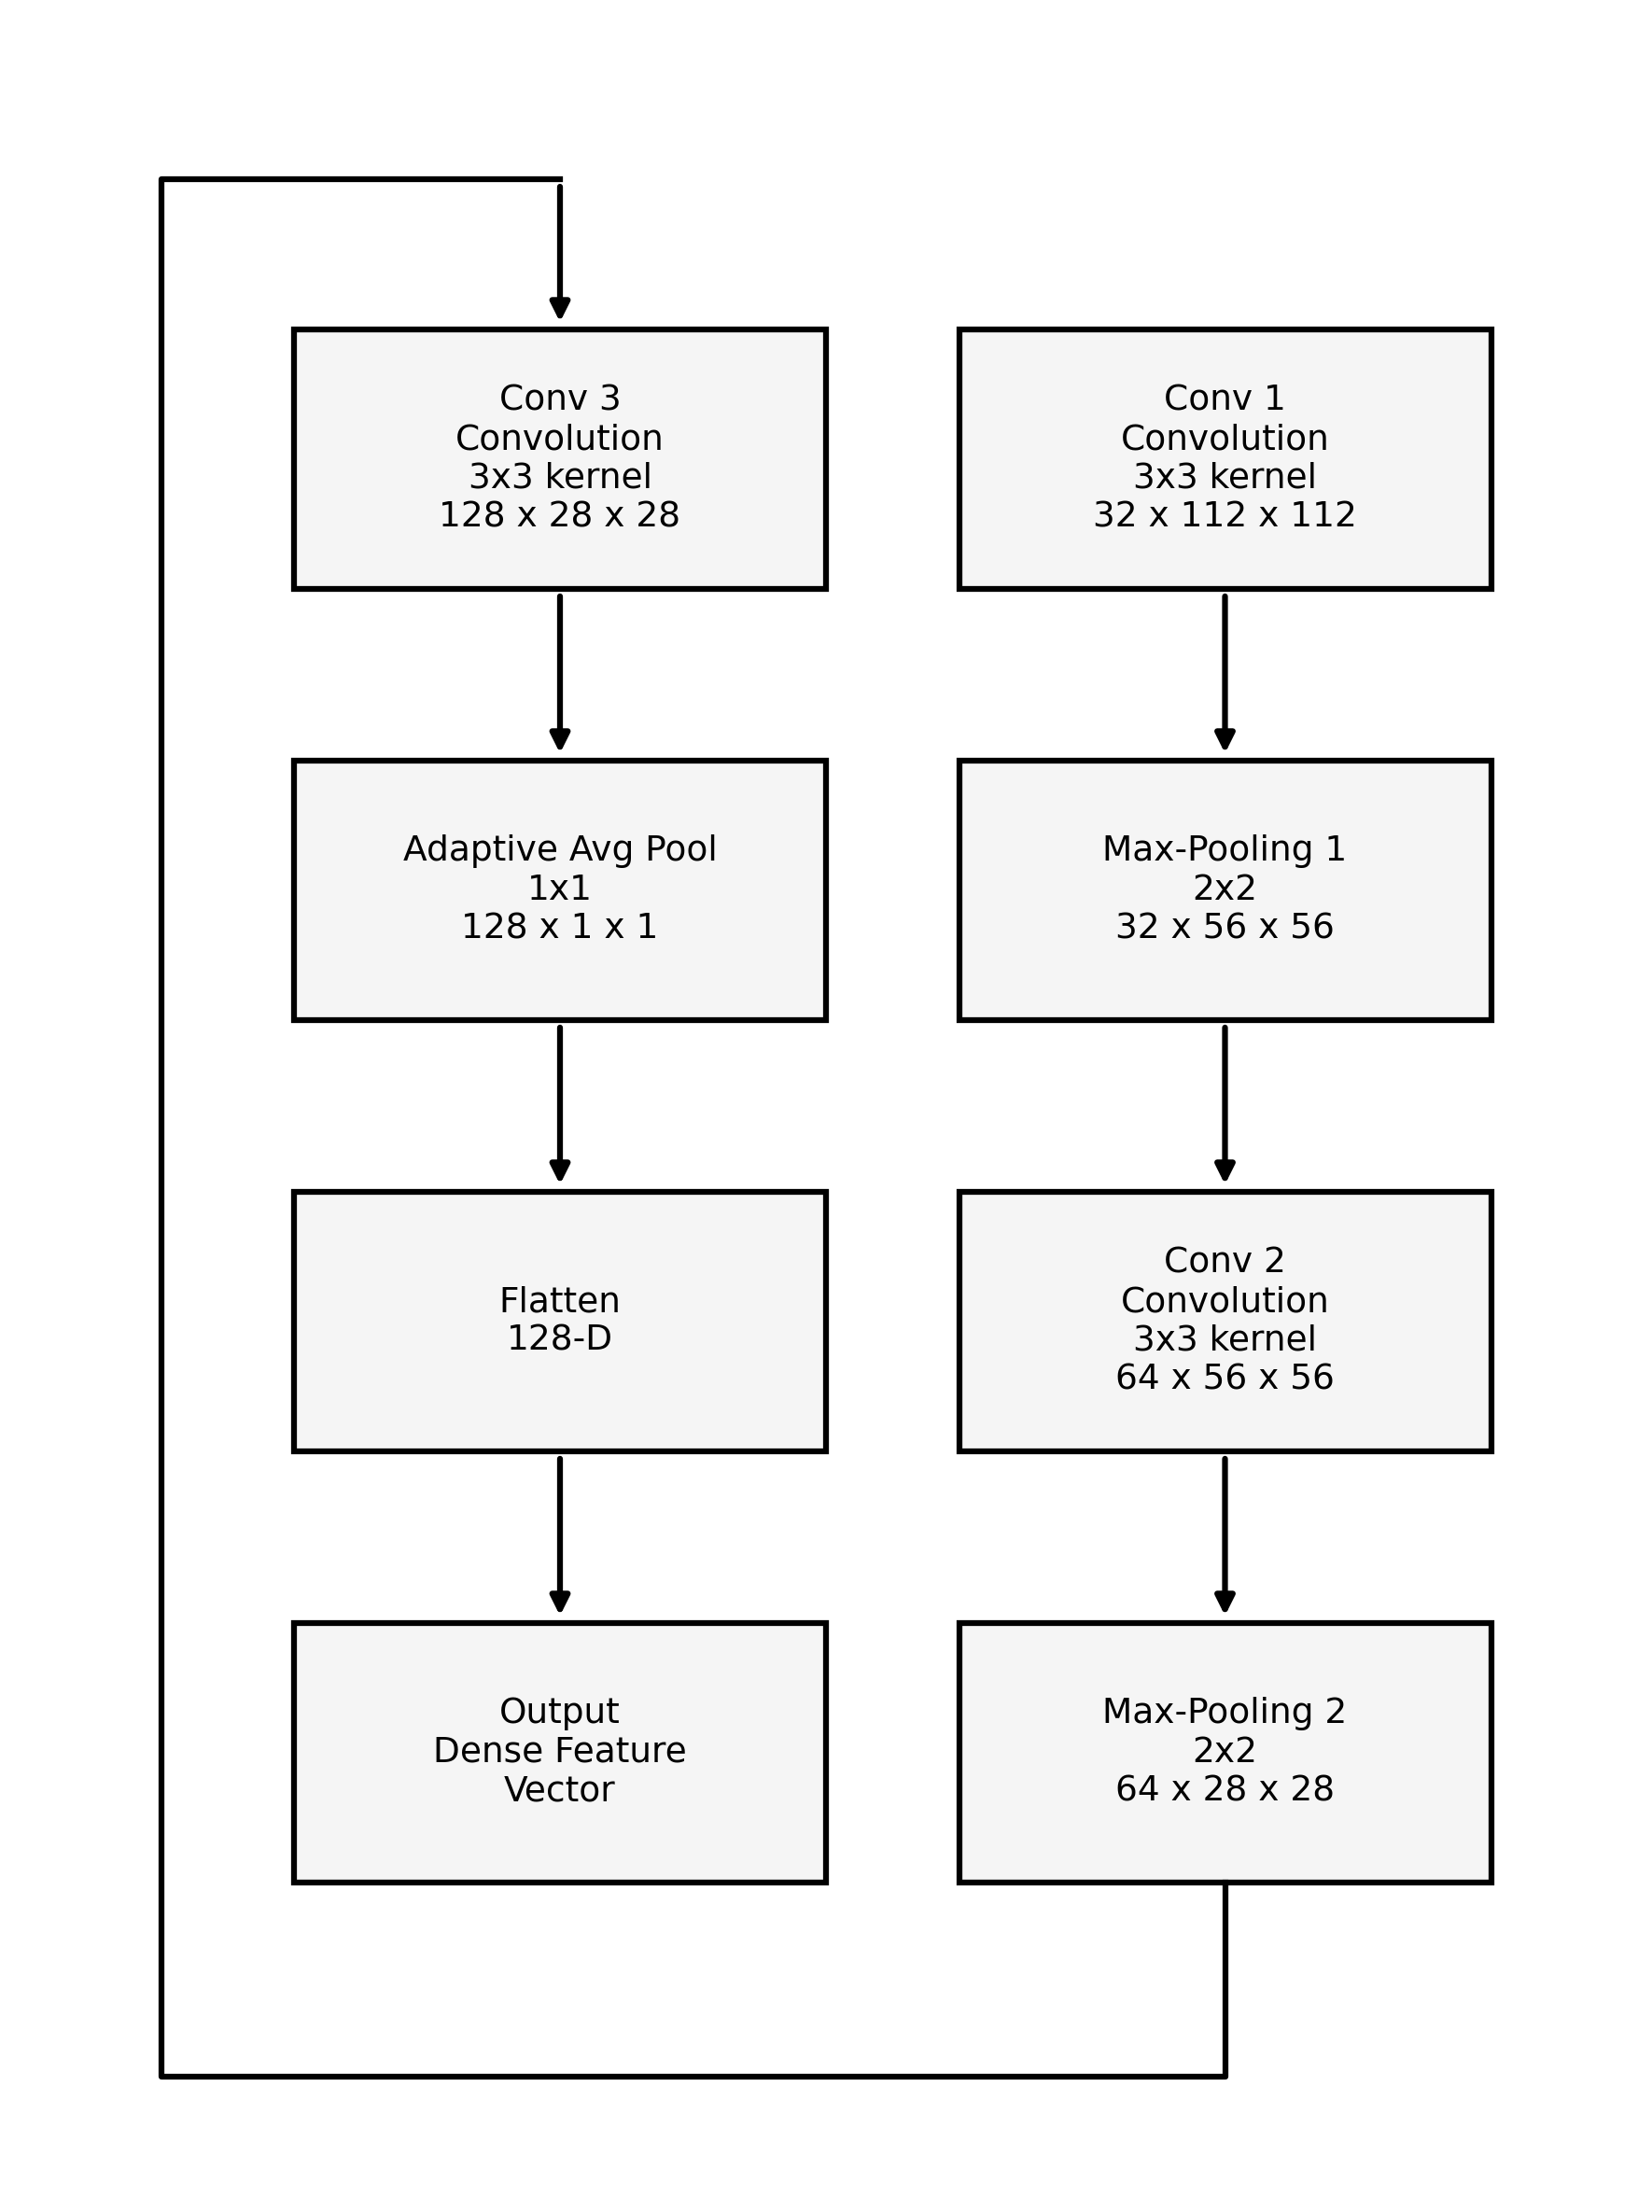
\includegraphics[width=0.6\textwidth]{images/pipeline.png}
\caption{CNN Architecture Pipeline}
\label{fig:pipeline}
\end{figure}

\subsection{Testing and Results}

The system underwent exhaustive testing using fresh guavas, rotten guavas, and unknown objects. 
\vspace{0.3cm}
\textbf{Fresh Detection:} When the system detects a fresh guava, the dashboard displays "ACCEPTED - FRESH", shows the confidence score, updates the freshness status, and records the prediction in the Inspection History.

\begin{figure}[H]
\centering
\includegraphics[width=0.8\textwidth]{images/screenshot1.png}
\caption{Fresh Guava Detection}
\label{fig:fresh}
\end{figure}

\vspace{0.3cm}
\textbf{Rotten Detection:} When the system detects a rotten guava, the dashboard displays "REJECTED - ROTTEN", shows the confidence score, automatically triggers the rotten alert sound, displays the alert indication on the dashboard, and records the prediction in the Inspection History.

\begin{figure}[H]
\centering
\includegraphics[width=0.8\textwidth]{images/screenshot2.png}
\caption{Rotten Guava Detection}
\label{fig:rotten}
\end{figure}

\vspace{0.3cm}
\textbf{Unknown Object Handling:} If the detected object is not recognized as a guava (for example, a Pear or an Apple), the application classifies it as "Unknown Object", displays the corresponding result and confidence score on the dashboard, and records the prediction in the Inspection History.

\begin{figure}[H]
\centering
\includegraphics[width=0.8\textwidth]{images/screenshot3.png}
\caption{Unknown Object Detection}
\label{fig:unknown}
\end{figure}

\vspace{0.3cm}
\textbf{Inspection History Management:} Every detection event is systematically logged in the Inspection History dashboard, ensuring complete traceability and allowing users to review all past predictions and confidence scores.

\begin{figure}[H]
\centering
\includegraphics[width=0.8\textwidth]{images/screenshot4.png}
\caption{Inspection History}
\label{fig:history}
\end{figure}

\subsection{Future Scope and Conclusion}

Future improvements to the system could include deploying the application on smaller devices, integrating it with a database to synchronize the inspection history, and expanding the AI model to support the detection of multiple fruit types.

In conclusion, the AI-Based Live Guava Freshness Detection System successfully achieves its objective of automating the inspection process. It demonstrates the practical application of AI and web development to solve real-world problems.
